%
% Footnotes
%
\def \naturalkey {Ein Schlüssel, der sich aus einem Attribut des Objekts ergibt oder sich aus mehreren Attributen zusammensetzt. So könnte ein sprechender Schlüssel von Jean-Luc Picard mit der E-Mail-Adresse picard@enterpise.com beispielsweise `picard@enterprise.com` (E-Mail) oder `Jean-LucPicard` (Zusammensetzung aus Vor- und Nachnamen) sein.}
\def \logicalclock {Eine Logische Uhr ist eine Komponente die dazu dient, dem Datenobjekt einen eindeutigen Zeitstempel zuzuweisen. Die bekanntesten Verfahren für Logische Uhren in verteilten Systemen sind die Lamport-Uhr und die Vektoruhr. Beide verwenden Zähler die sich bei jedem Ereignis erhöhen. Einfach gesagt besteht die Lamport-Uhr aus einem Zeitstempel und einem Zähler, die Vektoruhr aus einem Zeitstempel und einem Vektor -- einer Liste aus Zählern.}
%
%
\begin{description}[leftmargin=0.5cm,style=nextline]
  \item[Szenario ID0:]
  Zur Identifizierung eines Adressbucheintrags wird eine \gls{UUID} verwendet. Es wird sowohl auf dem Client als auch auf dem Server ein Kontakt mit dem Namen `Emilia Pond` erstellt. Währenddessen tritt Fall \it{b,c} ein und beide Parteien können nicht miteinander kommunizieren. Nach der Synchronisation existieren zwei Kontakteinträge mit gleichem Namen, aber unterschiedlicher ID. Sie sind voneinander zu unterscheiden und können einzeln behandelt werden.\\
  \item[Szenario ID1:]
  Zur Identifizierung eines Adressbucheintrags wird ein sprechender Schlüssel\footnote{\naturalkey} verwendet.
  Es wird sowohl auf dem Client als auch auf dem Server ein Kontakt mit dem Namen `Emilia Pond` und dem sprechenden Schlüssel `emiliapond` erstellt. Währenddessen tritt Fall \it{b,c} ein. Es ist nicht zu ermitteln, ob derselbe Kontakt doppelt angelegt wurde, wenn beide Kontakteinträge sich unterscheiden, welcher der beiden korrekt ist oder ob es sich bei den Einträgen um zwei Personen mit demselben Namen handelt.\\
  % Version
  \item[Szenario V0:]
  Zur Versionierung eines Adressbucheintrags werden Versionsnummern verwendet. Der Kontakt `Emilia` hat die Version `1.0.0`. Sowohl auf dem Client, als auch auf dem Server wird der Kontakt aktualisiert und geben ihm beide die Versonsnummer `2.0.0`. Währenddessen tritt Fall \it{b,c} ein und beide Parteien können nicht miteinander Kommunizieren. Bei der Synchronisation entsteht ein Konflikt weil es zwei (unterschiedliche) Einträge mit derselben Verion gibt.\\
  \item[Szenario V1:]% timestamp success
  Zur Versionierung eines Adressbucheintrags wird ein Zeitstempel verwendet. Der Kontakt `Emilia` hat die Version `2018-04-03 10:00:00Z`. Emilia ist umgezogen und ihre Adresse ändert sich. Der Eintrag wird bearbeitet und hat nun die Version `2018-04-13 11:44:22Z`. Während der Editierung tritt Fall \it{b,c} ein. Es stellt sich heraus, dass die Hausnummer einen Zahlendreher hat und es wird sofort berichtigt. `Emilia` hat nun die Version `2018-04-13 11:45:33`. Nach der Synchronisation gibt es nun zwei Objekte mit derselben ID: `Emilia` aber unterschiedlichen und zeitlich zuordenbaren Versionen. Durch den Zeitstempel ist sichergestellt, welcher Eintrag der neueste und wahrscheinlich korrekte ist.\\
  \item[Szenario V2:]% Timestamp fail
  Zur Versionierung eines Adressbucheintrags wird ein Zeitstempel verwendet. Das Szenario ist dasselbe wie \sc{V1} mit dem Unterschied, dass der Server eine spätere Uhrzeit als der Client hat. So hat nach der Synchronisation der später korrigierte Eintrag einen früheren Zeitstempel. Es wird die falsche, alte Adresse gespeichert, die korrekte hat einen älteren Zeitstempel und wird verworfen.\\
  \item[Szenario V3:]% Verktoruhr
  Zur Versionierung eines Adressbucheintrags wird eine Logische Uhr\footnote{\logicalclock} verwendet. Der Kontakt `Emilia` hat die Version \todo{Beispiel Logische Uhr?}. Emilias Telefonnummer ändert sich und wird auf dem Client angepasst (\todo{Version: }). Währenddessen tritt Fall \it{b, c} ein. Emilia sieht ihre falsche Telefonnummer und berichtigt diese ebenfalls. \todo{weil die Versionen identisch sind?} Bei der Synchronisation kommt es zum Konflikt. \todo{wirklich? auch wenn das Ergebnis dasselbe ist?}\\
  \item[Szenario V4:]% CAV
  % hash:  { name: Emilia Pond, phone: 0152397645, email: emilia@pond.com }
  Zur Versionierung eines Adressbucheintrags wird eine inhaltsbasierte Version verwendet. Um eine Zuordnung zwischen Inhalt und Version machen zu können kommen \Glspl{Hashfunktion} zum Einsatz. Hierbei wird als Version der Hashwert des Adressbucheintrags gespeichert.\\
  Der Kontakt `Emilia` hat die Version `5560348cec1b08c3d53e1508b4a46868`. Emilias Telefonnummer ändert sich und wird auf dem Client angepasst. Emilia sieht ihre falsche Telefonnummer und berichtigt diese zur gleichen Zeit. Da die Telefonnummer von beiden Parteien korrigiert wird und somit der Inhalt identisch ist, wird für beide Aktionen beide Version `88da3f8d82ab58551d2a48d74d9a4986` generiert. Es kommt zu keinem Konflikt, da die Versionen und der Inhalt identisch sind.\\
  \item[Szenario V5:]% CAV fail
  Zur Versionierung eines Adressbucheintrags wird eine inhaltsbasierte Version verwendet. Dem Kontakt `Emilia` ist die Version `5560348cec1b08c3d53e1508b4a46868` zugeordnet. Emilias Telefonnummer ändert sich und wird auf dem Client angepasst, während dieser \sc{offline} ist. Im selben Status berichtigt der Client die Telefonnummer. Bei der Synchronisation kommt es zum Konflikt, da es nun zwei Einträge mit unterschiedlichem Inhalt, aber identischer Version gibt und nicht festzustellen ist welche Version die neuere ist.\\
  \item[Szenario V6:] % CAV list
  Zur Versionierung eines Adressbucheintrags wird eine geordnete Liste von inhaltsbasierten Versionen verwendet.
  % So muss die Version nicht jedes Mal ersetzt werden und es ist sortierbar
  Dem Kontakt `Emilia` ist eine Liste von Verionen mit einem Eintrag `5560348cec1b08c3d53e1508b4a46868` zugeordnet. Emilias Telefonnummer ändert sich und wird auf dem Client angepasst, während dieser \sc{offline} ist. Im selben Status berichtigt der Client die Telefonnummer. Jede Aktion fügt der Versionsliste einen neuen Hashwert hinzu. Auch wenn der Content des Adresbucheintrags in den zwei letzten Versionen identisch ist, kann festgestellt werden welcher der neueste Eintrag ist. Kommt es zum Konflikt, werden die beiden \it{riskanten} Verionen verschachtelt in der Liste gespeichert. In diesem Fall sieht die Liste nun so aus: `[[88da3f8d82ab58551d2a48d74d9a4986, 88da3f8d82ab58551d2a48d74d9a4986], 5560348cec1b08c3d53e1508b4a46868]` -- eine Liste der beiden konfliktbehafteten Versionen am Anfang der Liste.
\end{description}
% \begin{figure}[H]
%   \centering
%   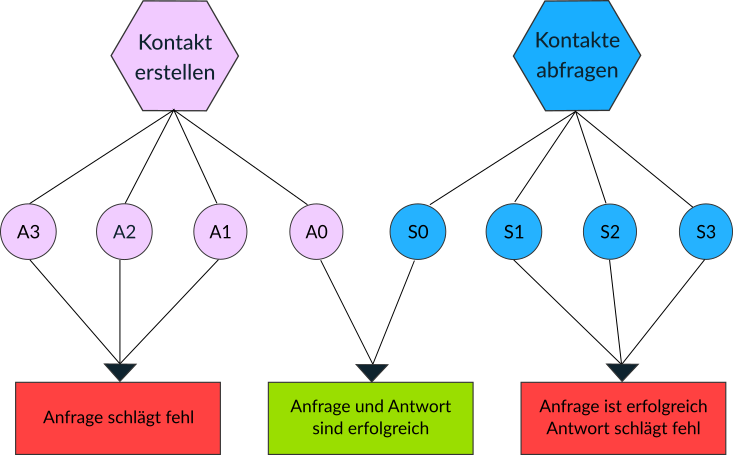
\includegraphics[width=0.8\textwidth]{Szenarien}
%   \grayRule
%   \caption[Szenarien]{Szenarien und Fälle}
%   \label{fig:scenarios}
% \end{figure}
%
% ERGEBNIS
%
\subsubsection*{Ergebnis}
Unterscheidung: Konflikt, nicht Konflikt\\
ID0 -- UUID und V3?, V6 als Gewinner.\\
Im weiteren Verlauf dieser Arbeit werden aus diesen Fällen die Anforderungen an eine offlinefähige Anwendung erarbeitet.